\section{Experiments}
\label{sec:exp}
We conduct experiments to investigate the behavior of the proposed multi-task selected learning BPP methods. As has been said above, our experiments are conducted on our 3D Bin Packing order data set L3DBPD.


\subsection{Implementation Details}
\label{sec:implementation}
Across all experiments, we use mini-batches of 128 sequences, LSTM cells with 128 hidden units, and embed the three coordinates of each item in a 128-dimensional space. We train our model with Adam optimizer \cite{kingma2014adam} with initial learning rate of $10^{-3}$ and decay every 5000 steps by a factor of 0.96. All the parameters are initialized randomly in $[-0.08,0.08]$ and clip $L2$ norm of our gradients to 1.0. We use the surface area calculated by heuristic algorithm NBPH as initial baseline input and apply $\alpha=0.7$ during the baseline iteration. We use 1000,000 steps to train the model and it will take about 70 hours on Tesla M40 GPU machine. Model implementation with TensorFlow will be made available soon.
Based on comprehensive consideration, the performance indicator is average surface area (ASA) which denotes the total cost of packing materials. The mathematical definition of ASA is as follows:
\begin{eqnarray*}
	ASA = \frac{\sum_{i=1}^{n} SA(i)}{n},
\end{eqnarray*}
where $SA(i)$ is the surface area of $i$th order and $n$ is the number of order.
 %\yu{No definition before, can be removed here and define in evaluation section.}
The experimental procedure and results are as follows.

%\noindent
\subsubsection{Multi-task Selected Learning Training}
For MTSL experiments, at each step, we choose a loss function of $\{L_{seq}, L_{ori}, L_{all}\}$ defined in section \ref{sec:train} at each batch adapting to the training process. Actually, we sample three loss with probabilities 0.3, 0.5, 0.2. The values of probabilities are annealed to 0.33, 0.33, 0.33 respectively over the first 10,000 training steps. Furthermore, we sample 800 times for each test instance and obtain the best as described in Section \ref{sec:test}. For comparison, we computed two kinds of ASA: 1) the sequence is generated by the sequence task and orientation is generated by the Algorithm \ref{Least surface Area Heuristic}; 2) the sequence and orientation are both generated by our MTSL model. We refer to those results as MTSL single-sample and MTSL multiple-sample.

\subsubsection{Reinforcement Learning Training}
In addition to the described methods, we also implement and train a pointer network with reinforcement learning similarly to \cite{Hu2017Solving} as the strong baseline method.
The stochastic policy of RL model is only related to the sequence of placing the items into bin, since other major factors are defined by the same heuristic algorithm NBPH mentioned above.
Previous work has already proved the effectiveness of this method against the heuristic method,
in which experiments shows that the reinforcement learning results with beam search at inference time are better than the NBPH baseline with an improvement of about $4.8\%$ \cite{Hu2017Solving}.
We regard it as strong baseline named RL vanilla-bs in our paper.
On the contrary, the vanilla method never takes the packing sequence that has already been produced into consideration.
We will empirically show the necessity of the introduced intra-attention mechanism through plenty of experiments and we refer this as RL intra-bs.
Consequently, the remaining experiments about RL models have introduced the intra-attention mechanism by default.
Furthermore, in order to carry out comparative test with the MTSL model, as our MTSL model adopts sampling strategy to obtain the best result at inference time, we also apply it in RL model. We call this approach RL single-sample. Meanwhile, to verify the effectiveness of probability distribution of orientations calculated by our MTSL model, we compare the results of the sequence generated by RL model following by random orientations, which is denoted as RL multiple-sample. %We refer to those approaches as RL vanilla-bs, RL intra-bs, RL single-sample and RL multiple-sample. \yu{I cannot distinguish them, maybe point out directly.}

%\noindent
\subsection{Results and Analysis}
\label{sec:eval}
%\kz{Generally, I feel the results are a bit slim. You have showed the main points in the contribution part of intro: intra-attention and sampling. What about multi-task? What if you don't use multi-task? Some kind of ablation tests? You can also show attention heat map to prove that attention works. Some results/error analysis will be helpful here.}
%We compare our methods against the heuristic baselines of increasing performance and complexity. NBPH method %is derived from the process of building blocks with Lego and 
%is based on idea of choosing the item, orientation and free space according to least waste space criteria, which aims to obtain least surface area at each step. The reason we choose it as a strong baseline is that it's the method deployed on operational system of Cainiao Supply Chain.  
%Among all the heuristic methods we have tested, the NBPH method has been proven to receive the least ASA. \yu{Any results?}
%Besides, the method deployed on operational system of Cainiao Supply Chain is similar to \cite{gonccalves2013biased}, where applying the same free space strategy. We called this method Random PSO.
%\yu{Very strange.}
%\yu{Besides, another baseline method is proposed by \cite{gonccalves2013biased}, it will apply the same free space strategy. }

First of all, we evaluate different models including RL vanilla-bs and RL intra-bs on our proposed dataset L3DBPD. We report the ASA in Table \ref{rl result}.
As the table shows, the RL vanilla-bs achieves $4.89\%$, $4.88\%$, $5.33\%$ improvement than NBPH for BIN8, BIN10 and BIN12, whereas the improvement of the RL intra-bs is increased to $5.19\%$, $5.26\%$, $5.41\%$ instead. Apparently, this demonstrates the usefulness of our intra-attention training method for New 3D BPP which can help reduce the surface area.
Besides, we also conduct the approach BRKGA in \cite{gonccalves2013biased} on L3DBPD to validate whether these method designed for fixed-sized bin are appropriate for our new 3D BPP.
BRKGA is one of the state-of-the-art method to tackle 2D and 3D fixed-sized bin packing problems which adopts a heuristic method of Genetic Algorithm.
According to Table \ref{rl result}, we find that BRKGA is dramatically limited by the non-fixed-sized bin. It even performs worse than the random method which randomly generates the packing sequence and adopts the orientation and free space calculated by Algorithm \ref{Least surface Area Heuristic}. All in all, the statistical analysis confirms that RL intra-bs is significantly better than all the other approaches outlined below.

\begin{table}[!htb]
	\centering
	\caption{Comparison with RL vanilla-bs and RL intra-bs on the L3DBPD Dataset.  }
	\label{rl result}
	\begin{tabular}{l|l l l}
		\hline
		model &   BIN8 & BIN10 & BIN12 \\ \hline
		Random &  44.70 & 48.38 & 50.78 \\ 
		NBPH method & 43.97 & 47.33 & 49.34 \\
		BRKGA  &59.44 & 65.73 & 68.47 \\
		RL vanilla-bs & 41.82 & 45.02 & 46.70 \\ 
		RL intra-bs & \textbf{41.69} & \textbf{44.84} & \textbf{46.67} \\ \hline
	\end{tabular}
\end{table}

Thus, we report the ASA of our rest approaches on BIN8, BIN10, and BIN12 in Table \ref{bin result}. Notably, results demonstrate that training with RL and MTSL significantly comfortably surpass the NBPH method. By calculation, the proposed MTSL multiple-sample achieves $6.21\%$, $7.80\%$, $8.55\%$ improvement than NBPH method for BIN8, BIN10, and BIN12. In our experiments, MTSL multiple-sample proves superior than other methods in most cases but is slightly less competitive than RL single-sample in BIN8.

\begin{table}[!htb]
	\centering
	\caption{ASA of mentioned methods, and all ASA are obtained of 1000 times sampling. }
	\label{bin result}
	\begin{tabular}{l|l l l}
		\hline
		model &   BIN8 & BIN10 & BIN12 \\ \hline
		Random &  44.70 & 48.38 & 50.78 \\ 
		NBPH method & 43.97 & 47.33 & 49.34 \\ 
		MTSL single-sample & 42.25 & 44.34 & 45.30 \\ 
		MTSL multiple-sample & 41.24 & \textbf{43.64} & \textbf{45.12} \\ 
		RL single-sample & \textbf{41.12} & 44.03 & 45.58 \\ 
		RL multiple-sample & 41.21 & 45.01 & 47.42 \\ \hline
	\end{tabular}
\end{table}

We present a more detailed comparison of our methods in Figure \ref{fig:curve-model}, where we show the relationship between their performances and corresponding sampling times. The curve reveals a fact that MTSL multiple-sample approach which produces the sequence and orientations simultaneously outperforms other learning configurations in most cases. The contrast between RL multiple-sample and MTSL multiple-sample demonstrably illustrates that the probability distribution of orientations calculated by our MTSL model is indeed effective, as the ASA with MTSL significantly improves over RL. Furthermore, we find that the orientation task can definitely promote better results, even though the MTSL multiple-sample is just a few percents worse than NBPH baseline and MTSL single-sample at the very beginning. Moreover, MTSL multiple-sample approach benefits from much less orientation search space and run efficient than the methods that adopt the heuristic orientation calculation which will search from $6^n$ space at most.
%\begin{figure}[h]
%	\centering
%	\subfigure[]{\includegraphics[width=0.49\columnwidth]{figure/BIN8.pdf}} \hfill
%	\subfigure[]{\includegraphics[width=0.49\columnwidth]{figure/BIN10.pdf}}\\
%	\subfigure[]{\includegraphics[width=0.49\columnwidth]{figure/BIN12.pdf}}
%	\caption{Results for multi-task binpacking network. (a), (b), (c) shows the result of BIN8, BIN10, BIN12, respectively.}
%	\label{fig:curve-model}
%	\vspace{-10pt}
%\end{figure}
%
\begin{figure*}[h]
	\centering
	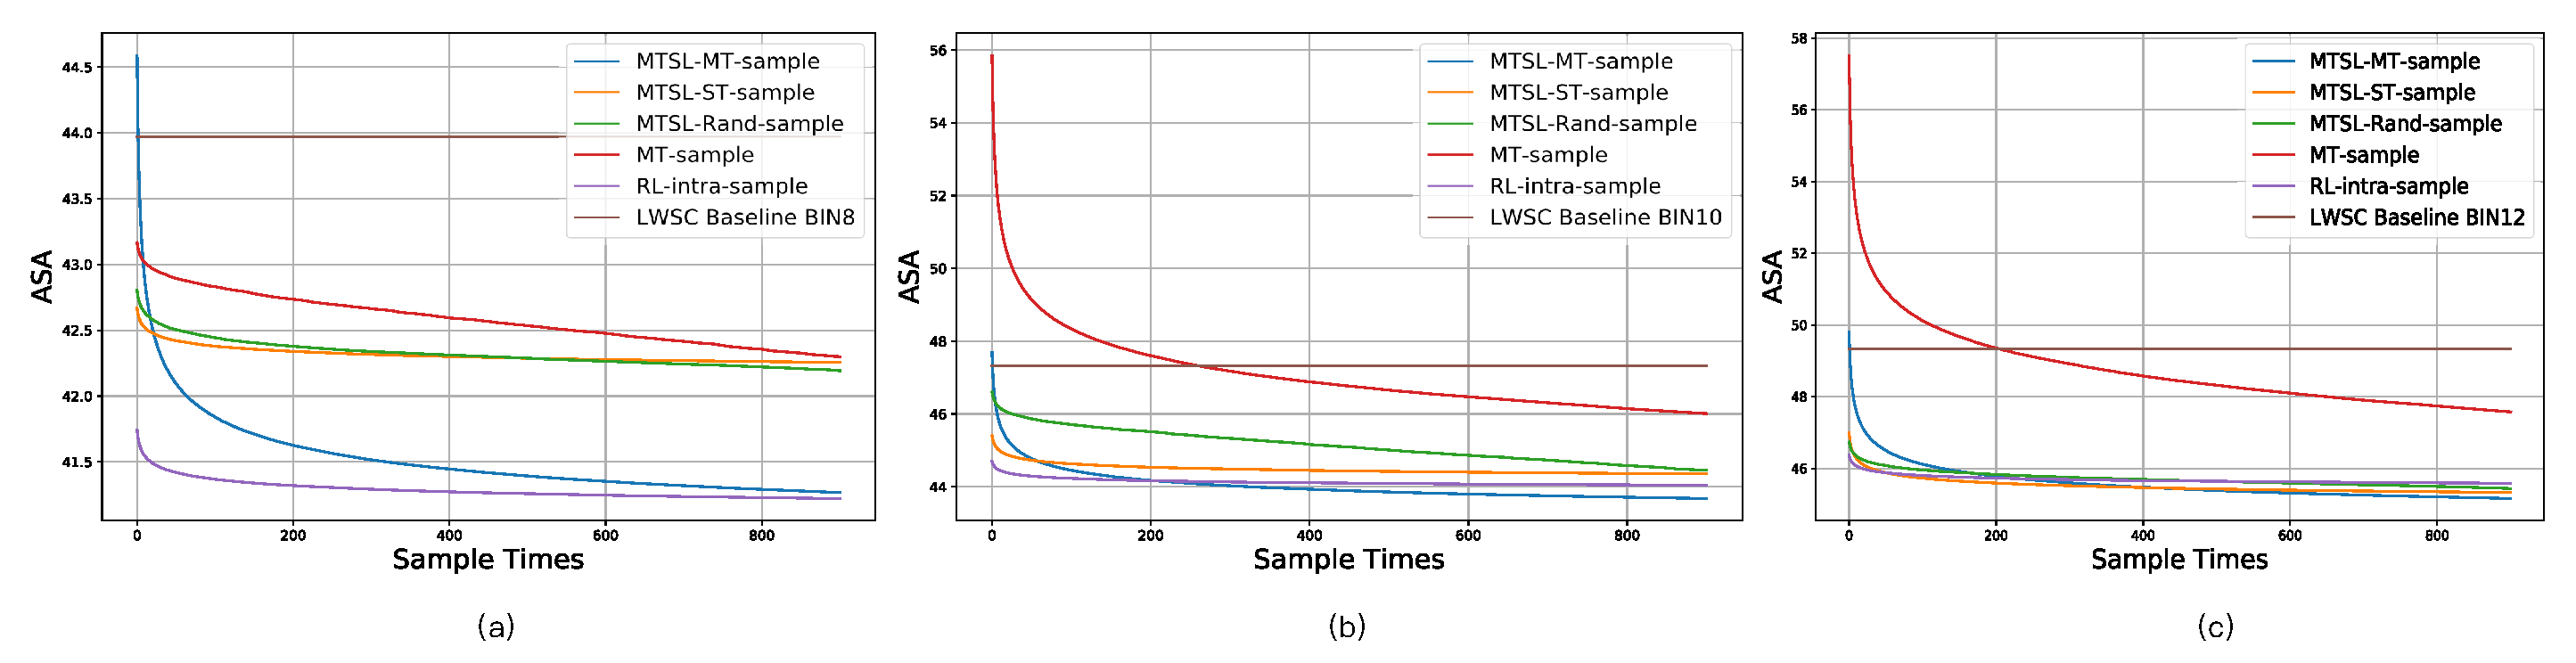
\epsfig{file=binresult.pdf, width=2.1\columnwidth}
	\caption{Results for multi-task binpacking network. (a), (b), (c) shows the result of BIN8, BIN10, BIN12, respectively.}
	\label{fig:curve-model}
	\vspace{-10pt}
\end{figure*}

Finally, we randomly pick an example order and produce results by different methods in Figure \ref{fig:result-example} for case study. The example order is from BIN8 and the results are obtained by sampling 500 times.
As shown, the surface area computed by each method is listed on the top of each results. Obviously, the computational experiment results demonstrate that MTSL multi-sample can produce a more reasonable packing policy than other methods. 

%\begin{figure}[h]
%	\centering
%\subfigure[SL %single-sample]{\includegraphics[width=0.48\columnwidth]{figure/SL-single-sample.pdf}} \hfill
%\subfigure[SL multiple-sample]{\includegraphics[width=0.48\columnwidth]{figure/SL-multiple-sample.pdf}}\\
%\subfigure[RL single-sample]{\includegraphics[width=0.48\columnwidth]{figure/RL-single-sample.pdf}}\hfill
%\subfigure[RL multiple-sample]{\includegraphics[width=0.48\columnwidth]{figure/RL-multiple-sample.pdf}}\\
%\subfigure[NBPH Method]{\includegraphics[width=0.48\columnwidth]{figure/NBPH			Method.pdf}}
%	\caption{Sampled result of bpp. NBPH method result and SL single-sample, SL multiple-sample, RL single-sample, RL multiple-sample.}
%	\label{fig:result-example}
%	\vspace{-10pt}
%\end{figure}

\begin{figure}[h]
	\centering
	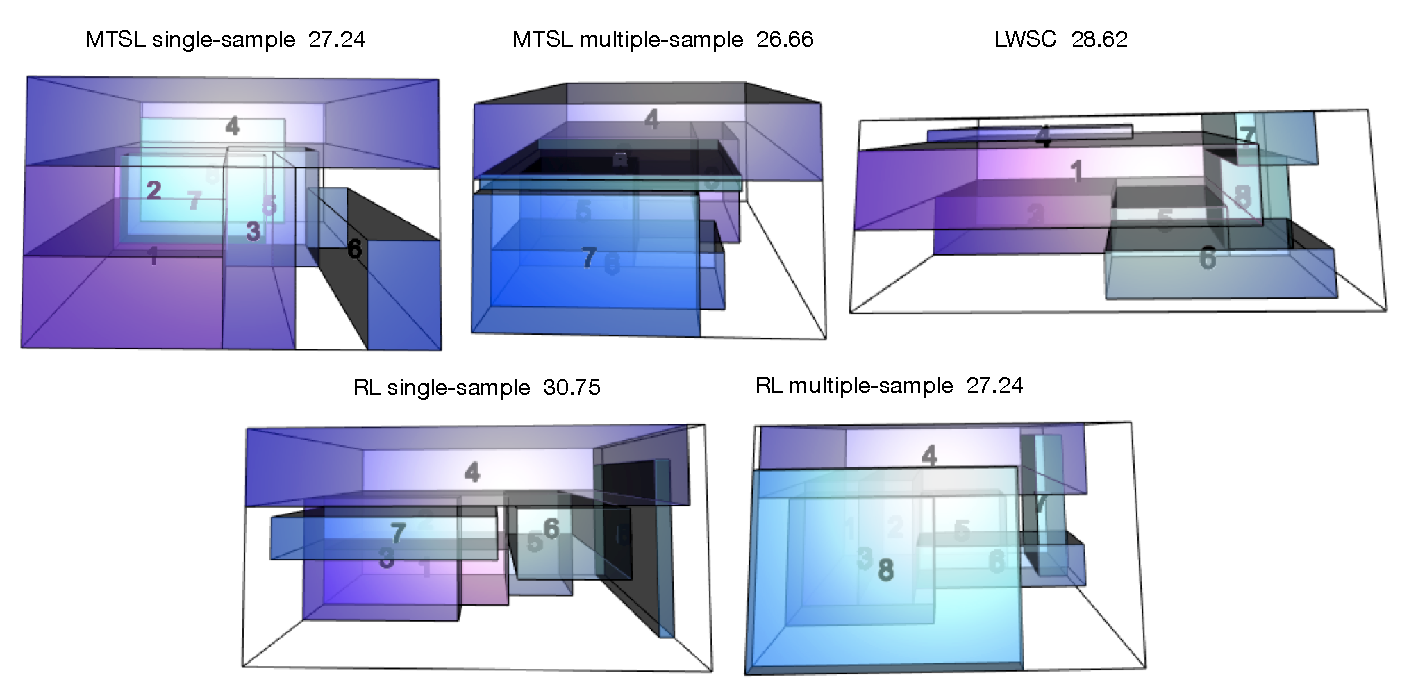
\epsfig{file=binpacking_result.eps, width=0.95\columnwidth}
	\caption{Results of MTSL single-sample, MTSL multiple-sample, RL single-sample, RL multiple-sample and NBPH method. The surface area of these method are 27.24, 26.66, 30.75, 27.24 and 28.62 respectively}
	\label{fig:result-example}
	\vspace{-10pt}
\end{figure}
